\section{Bayesian Networks (part 1/2)}



\mode<presentation>{
\begin{frame} 
    \begin{center} \huge
        \secname
    \end{center}
    \begin{center}   
    Towards an efficient representation of the full joint distribution that exploits conditional independence
    \end{center}
\end{frame}
}



% =============================================================================
\subsection{Directed Acyclic Graphs (DAG)}


\begin{frame}\frametitle{\subsecname}

A graphical representation of conditional independence:
\begin{figure}[h]
	\centering
	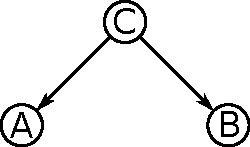
\includegraphics[width=0.3\linewidth]{img/cond}%
	\notesonly{
	\caption{
	The conditional independence between $A$ and $B$ given $C$.
	}%
	}%
    \label{fig:cond}%
\end{figure}

This leads to the factorization of the full joint distribution:

\begin{equation}
P(A,B,C) = P(A|C)P(B|C)P(C)
\end{equation}

\end{frame}


\begin{frame}\frametitle{\subsecname}
    
\question{What does the DAG representation of this full joint distribution look like for toothache example?}

(\textbf{see blackboard})

\end{frame}

\subsubsection{A ``Californian'' example}

% -----------------------------------------------------------------------------
\begin{frame} \frametitle{\subsubsecname}
	\begin{center}
	\slidesonly{
		\includegraphics<1>[width=7cm]{img/section3_fig5_v2_1} 
		}
%		\includegraphics<2>[width=8cm]{img/section3_fig5_v2_2}
		\includegraphics<2>[width=7cm]{img/section3_fig5_v2_2}  
	\end{center}
	
%	\only<2>{
%	\begin{itemize}
%		\item set of random variables 
%			$\leadsto$ nodes of the graph
%		\item direct influences between variables 
%			$\leadsto$ directed links between nodes
%		\item nodes $x_i$ are annotated with the conditional probabilities\\
%			\quad$P\big(X_i\,|\, \text{parents}(X_i)\big)$
%	\end{itemize}
%	} 
Considering statistical dependencies, only 10 instead of 31 entries have to be stored.
	{ \small
		\begin{align} 
			P(J,M,A,B,E) \stackrel{\substack{\text{product}\\\text{rule}}}{=}& 
			P(J|M,A,B,E) \, P(M|A,B,E) \, P(A|B,E) \, P(B|E) \, P(E) \\\slidesonly{\vspace{-5mm}}
			\stackrel{\substack{\text{cond.}\\\text{indep.}}}{=}& P(J|A) \, P(M|A) \, P(A|B,E) \, P(B) \, P(E)
		\end{align}
	}
\end{frame}

%\begin{frame} \frametitle{A ``Californian'' example: Inferemce}
	%\begin{center}
		%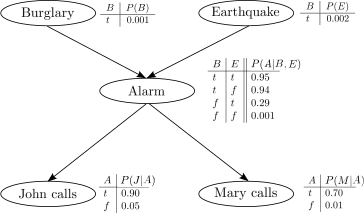
\includegraphics[width=7.5cm]{img/section3_fig5_v2_2}  
	%\end{center}
	

%\begin{equation}
	%\begin{array}{lll}
	%P(B|J=true, M=true) 
	%& = & \underbrace{ \alpha P(B, J=true, M=true) }_{
		%\substack{ \text{normalization} \\ \text{c.f. section 3.1.3}}} \\\\
	%& = & \underbrace{ \alpha \sum\limits_{a,e} P(B, e, a, 
				%J=true, M=true) }_{
		%\text{marginalization}} \\\\
	%& = & \alpha P(B) \sum\limits_e P(e) \sum\limits_a P(a|B,e) \\
	%&& \cdot P(J=true|a) P(M=true|a) \\\\
	%& = & \alpha \cdot \left \{ \begin{array}{ll}
			%0.00059224 & \text{for } B=true \\\\
			%0.0014919 & \text{for } B=false
		%\end{array} \right.
	%\end{array}
%\end{equation}
%\end{frame}

\begin{frame}\frametitle{\secname}
    
A factorization of the full joint distribution\footnote{See Ch. 14 from \citep{russell2016artificial} for more details.}:

\begin{equation}
P(X_{1},\ldots,X_{n}) = \prod_{i=1}^{n} P(X_{i} | parents(X_{i}))
\end{equation}
    
Remember: independence is important. Independence can be identified via the 
\underline{Markov blanket}

The Markov blanket of a node includes:
\begin{itemize}
\item its parents
\item its children
other parents of the children    
\end{itemize}
    
\end{frame}

\subsection{Preparations to perform inference}

\begin{frame}\frametitle{\subsecname}
    
    \begin{enumerate}
     \item use topological representation to ensure a compact representation.
     The purpose of topological sorting is to identify cliques in the chordal decomposable graph (next week)
     \item turn DAG into a \emph{moral graph} i.e. \\
     an undirected graph + new edges s.t. each node of the original DAG is now directly connected to the nodes of its \emph{Markov blanket}
     \item Perform inference efficiently (next week)\\
     \textcolor{gray}{ by applying \emph{message passing} on the \emph{Junction tree}}
    \end{enumerate}
    
\end{frame}

\subsubsection{Topological sorting}


% -----------------------------------------------------------------------------
\begin{frame} \frametitle{\subsubsecname}

\mode<presentation>{
	\begin{textblock}{}(10.5,10)
		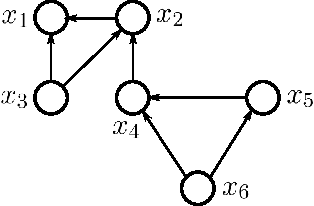
\includegraphics[width=4cm]{img/section3_fig17}
	\end{textblock}
	}

	\begin{itemize}
	\mode<presentation>{
		\item Factorization of the unconditional probability:
		$$
				P(X_1,\ldots, X_n) \quad=\quad 
				{\textstyle\prod\limits_{i=1}^n} P\big(X_i\,|\,parents(X_i)\big)
		$$
		\vspace{4mm}
		}
		
\mode<article>{
	\begin{figure}[h]
		 \centering
		 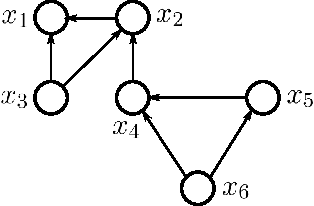
\includegraphics[width=0.4\textwidth]{img/section3_fig17}%
		 \caption{Example DAG}
	\end{figure}
}
		\item Edges should always be directed from nodes with lower 
			to nodes with higher indices.
		\vspace{8mm}
		\item Topological sorting: From parents to children:
			\begin{enumerate}
				\item select and queue a node without parents
				\item delete that node from the DAG
				\item repeat until DAG is empty
				\item renumber nodes
			\end{enumerate}
	\end{itemize}
\end{frame}


% -----------------------------------------------------------------------------
\begin{frame} \frametitle{\subsubsecname}
	\begin{minipage}{12.1cm}
		\begin{minipage}{7cm}
			\begin{itemize}
				\item example:
					\begin{itemize}
						\item ${\color{red}x_3},
							\visible<2->{x_6,}
							\visible<3->{x_5,}
							\visible<4->{x_4,}
							\visible<5->{x_2,}
							\visible<6->{x_1}$
					\end{itemize}
				\vspace{5mm}
				\item<7-> other possible topological orderings:
					\begin{itemize}
						\item $x_6,
							\visible<2->{x_5,}
							\visible<3->{x_4,}
							\visible<4->{{\color{red}x_3},}
							\visible<5->{x_2,}
							\visible<6->{x_1}$
						\item $x_6,
							\visible<2->{x_5,}
							\visible<3->{{\color{red}x_3},}
							\visible<4->{x_4,}
							\visible<5->{x_2,}
							\visible<6->{x_1}$
						\item $x_6,
							\visible<2->{{\color{red}x_3},}
							\visible<3->{x_5,}
							\visible<4->{x_4,}
							\visible<5->{x_2,}
							\visible<6->{x_1}$
					\end{itemize}
			\end{itemize}
		\end{minipage}
		\begin{minipage}{4cm}
			\includegraphics<1>[width=4cm]{img/section3_fig17_step1}
			\includegraphics<2>[width=4cm]{img/section3_fig17_step2}
			\includegraphics<3>[width=4cm]{img/section3_fig17_step3}
			\includegraphics<4>[width=4cm]{img/section3_fig17_step4}
			\includegraphics<5>[width=4cm]{img/section3_fig17_step5}
			\includegraphics<6>[width=4cm]{img/section3_fig17_step6}
			\mode<presentation>{
			\includegraphics<7>[width=4cm]{img/section3_fig17}
			}
		\end{minipage}
	\end{minipage}
\end{frame}

\begin{frame}

Exercise: topological sorting

\begin{figure}[h]
	\centering
	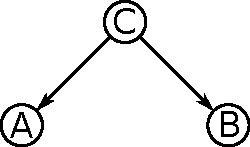
\includegraphics[width=0.3\linewidth]{img/cond}%
	\notesonly{
	\caption{
	DAG
	}%
	}%
    \label{fig:cond}%
\end{figure}

	\begin{itemize}
		\item Topological sorting: From parents to children:
			\begin{enumerate}
				\item select and queue a node without parents
				\item delete that node from the DAG
				\item repeat until DAG is empty
				\item renumber nodes
			\end{enumerate}
	\end{itemize}


\textbf{(see blackboard)}


\end{frame}


\begin{frame}

Exercise: topological sorting

\begin{figure}[h]
	\centering
	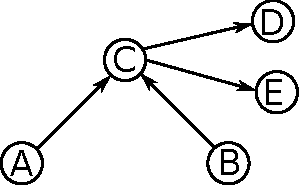
\includegraphics[width=0.3\linewidth]{img/dag1}%
	\notesonly{
	\caption{
	DAG
	}%
	}%
    \label{fig:cond}%
\end{figure}
\mode<presentation>{
	\begin{itemize}
		\item Topological sorting: From parents to children:
			\begin{enumerate}
				\item select and queue a node without parents
				\item delete that node from the DAG
				\item repeat until DAG is empty
				\item renumber nodes
			\end{enumerate}
	\end{itemize}
}

\textbf{(see blackboard)}


\end{frame}

\begin{frame}

Exercise: DAG (same as before) to moral graph

\mode<presentation>{
\begin{figure}[h]
	\centering
	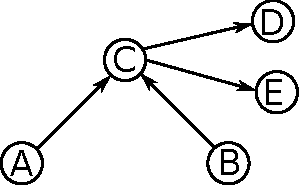
\includegraphics[width=0.3\linewidth]{img/dag1}%
	\notesonly{
	\caption{
	DAG
	}%
	}%
    \label{fig:cond}%
\end{figure}
}
\mode<presentation>{
\begin{enumerate}
\item make the edges undirected
\item identify the Markov blanket of each node (parents, children, other parents of the children)
\item add edges such that all nodes are directly connected to the Markov blanket.
\end{enumerate}
}

\textbf{(see blackboard)}
    
\end{frame}
